\documentclass[a4paper, punct,space,nospace, fancyhdr, fntef,UTF8]{ctexart}


\usepackage{szutils}%在这里放置需要的宏包,并设置部分所需内容

\begin{document}

	\pagestyle{empty}%不要页眉页脚
	%封面与诚信声明
	
%\centerline{\kaishu\zihao{-0}{深圳大学}}
\begin{figure}[htbp]
	\begin{center}
		\includegraphics[width=2.7in]{szu}
	\end{center}
\end{figure}


\centerline{\heiti\zihao{1}{本\ 科\  毕\  业\  论\  文\  (设计)}}

\vskip 3.5cm



\begin{flushleft}
	\zihao{3}
	\hspace{3cm}{\heiti{题目:}}      
	{\kaishu\underline{\quad\textbf{融合内容信息的单类协同}\hspace{1.2cm}}}               \\
	\vspace{10bp}
	\hspace{3cm}{\kaishu\underline{\hspace{2.7cm}\quad\textbf{过滤推荐算法研究}\hspace{2.1cm}}}
	\vspace{10bp}
	
	\hspace{3cm}{\heiti{姓名:}}      
	{\kaishu\underline{\hspace{2.8cm}\textbf{徐留成}\hspace{3.5cm}}}              \\
	\vspace{10bp}
	
	\hspace{3cm}{\heiti{专业:}}     
	{\kaishu\underline{\hspace{1.5cm}\textbf{计算机科学与技术}\hspace{2cm}}}            \\
	\vspace{10bp}
	
	\hspace{3cm}{\heiti{学院:}}      {\kaishu\underline{\hspace{1.5cm}\textbf{计算机与软件学院}\hspace{2cm}}}               \\
	\vspace{10bp}
	
	\hspace{3cm}{\heiti{学号:}}      {\kaishu\underline{\hspace{2.4cm}\textbf{2012080173}\hspace{2.6cm}}}                   \\
	\vspace{10bp}
	
	\hspace{3cm}{\heiti{指导教师:}} 
	{\kaishu\underline{\hspace{1.8cm}\textbf{潘微科}\hspace{3.5cm}} }                         \\
	\vspace{10bp}
	
	\hspace{3cm}{\heiti{职称:}}      
	{\kaishu\underline{\hspace{3.2cm}\textbf{讲师}\hspace{3.8cm}} }                         \\
	
\end{flushleft}

\vskip 4cm

\centerline{\zihao{3} 2016 年 \  4 月\  27 日}
	\newpage

\centerline{\heiti\zihao{-2}{深圳大学本科毕业论文(设计)诚信声明}}


\vskip 3cm 


\begin{spacing}{2.0}
	\zihao{4}
本人郑重声明:所呈交的毕业论文(设计),题目《融合内容信息的单类协同过滤推荐算法研究》是本人在指导教师的指导下,独立进行研究工作所取得的成果。对本文的研究做出重要贡献的个人和集体,均已在文中以明确方式注明。除此之外,本论文不包含任何其他个人或集体已经发表或撰写过的作品成果。本人完全意识到本声明的法律结果。

\vskip 3cm

{\flushright{
		毕业论文(设计)作者签名:\hspace{2.2cm}
		
		
		
		\hspace{7.5cm}{日期:\hspace{2cm}年 \hspace{.5cm}月\hspace{.5cm}日}\hspace{4cm} 
	}}
\end{spacing}



	
	
	\zihao{-4}
	\tableofcontents%生成目录
	\thispagestyle{empty}%页脚不要页码
	%“目录”两个字的样式与section的样式一致,默认居中,故将设置section标题居左放置在生成目录后
	\CTEXsetup[format={\Large\bfseries}]{section}  %section标题居左
	
	%%%%正文开始,页脚有页码
	\cfoot{\zihao{-5}第 \ \thepage \ 页 \ 共 \ \pageref{lastpage} 页}%%%%lastpage为末页标签
	%正文
	\zihao{5}
	\pagenumbering{arabic}%页码使用阿拉伯数字
	\setcounter{page}{0}  %重新设置页码计数
	\pagestyle{fancy}
	
	\newpage


\centerline{\fangsong\bf\zihao{-2}{融合内容信息的单类协同过滤推荐算法研究}}
\addcontentsline{toc}{section}{摘要(关键词)}%加入目录


\vskip 1cm

\begin{center}
	\kaishu
	\hspace{2cm}计算机与软件学院计算机科学与技术专业 \quad 徐留成 
	\vspace{5bp}
	\newline
	学号:2012080173
\end{center}

\vskip 10bp

{
\kaishu	
\hspace{5bp}{\zihao{-4}\textbf{【摘要】}} 
对于基于隐式反馈的个性化推荐算法而言,pairwise learning是一个非常重要的技术手段。pairwise learning 算法通常基于这样一个假设:对一个用户而言,相比于未选择过的物品往往会更感兴趣于已选择过的物品。这种假设在推荐算法的学习过程中会衍生出大量的training pairs。而为了应对大规模的数据集,我们所研究的推荐算法往往都是基于均匀采样的随机梯度下降方法进行求解。不过,这种采取均匀采样的策略经常会导致算法收敛非常缓慢。在本文中首先讨论了均匀采样策略导致收敛缓慢的原因,并研究了通过在已有的BPR推荐框架中融合内容信息 改进采样策略并最终提高推荐效果的方法。实验证明,相比于均匀采样策略,通过融合内容信息的适应性采样策略的确能够有助于提高推荐效果。

\vskip 10bp

\hspace{5bp} {\zihao{-4}\textbf{【 关键词】}} 
推荐系统; 协同过滤; 适应性采样  
}
	\section{引言}

\subsection{研究背景及意义}

互联网的出现和普及给用户带来了大量的信息, 满足了用户在信息时代对各种信息的需求, 但随着Internet的迅速发展而带来的网络上信息量的巨幅增长, 使得用户在面对大量信息时无法快速从中获得对自己真正有用的那部分信息。换言之, 在这种情况下人们对信息的使用效率反而降低了, 这就是所谓的信息过载(information overload)问题. 的确如此, 面对信息的汪洋大海, 人们往往感到无所适从, 信息过载已经成为一个不容忽视的问题.

目前, 应对信息过载的办法之一便是以搜索引擎为代表的信息检索系统, 比如国外的Google\footnote{\url{https://www.google.com/}}、国内的Baidu\footnote{\url{https://www.baidu.com/}}等, 它们在帮助用户从巨大的网络资源中获取信息方面发挥着极其重要的作用. 但对于使用搜索引擎的用户而言, 在使用同一个关键字搜索信息时, 在一段时间内所得到的结果都是相同的. 另一方面来看,信息及其传播是多样化的, 而用户对信息的需求是多元化和个性化的, 那么通过以搜索引擎为代表的信息检索系统获得的结果显然不能满足用户的个性化需求, 它们仍然无法很好地解决信息过载问题.

面对信息过载, 另外一个非常有潜力的办法是个性化的推荐系统, 它是根据用户的信息需求、兴趣等, 将用户所感兴趣的信息、产品、服务等推荐给用户的个性化信息推荐系统. 和搜索引擎相比, 推荐系统通过研究用户的历史行为与兴趣偏好, 进行个性化考量, 由系统发现用户的兴趣点, 从而引导用户发现自己的信息需求. 一个优秀的推荐系统不仅能为用户提供个性化的服务, 还能和用户之间建立密切关系, 让用户对其推荐产生依赖. 个性化推荐系统现已广泛应用于很多领域, 其中最典型并具有良好的发展和应用前景的领域就是电子商务领域. 目前,几乎所有大型的电子商务系统,如 Amazon, eBay, 京东, 当当网上书店等, 都不同程度地使用了各种形式的推荐系统。同时学术界对推荐系统的研究热度一直很高, 逐步形成了一个独立的研究领域.

Internet为人们提供了极其丰富的信息资源,在这些海量、异构的Web信息资源中蕴含着具有巨大潜在价值的知识。根据用户访问的历史记录以及各种服务或商品之间的相关信息可以构建用户的兴趣模型,从而凭借该用户的兴趣模型对繁杂的信息进行过滤, 然后向用户推荐其可能感兴趣的服务或商品。事实上, 推荐系统已经成为目前解决信息过载最有效的工具之一。




\subsection{本文主要工作}

本文从推荐系统的概述展开, 讨论了在推荐系统的学习算法中随机梯度下降方式中采用均匀采样策略而导致收敛缓慢的一些原因, 并通过融合内容信息改进了均匀采样策略--适应性采样策略, 然后将适应性采样策略放入已有的推荐算法框架中, 加快原有推荐算法的学习。




\subsection{论文组织结构}

 本论文共分为七章,内容如下: 

 第一章为引言, 主要介绍了本论文的研究背景、意义, 主要工作及论文的组织结构.
 
 第二章为推荐系统概览,并分类介绍了包括了基于内容、基于系统过滤与混合型推荐算法的一些典型的推荐学习算法。
 
 第三章为预备工作,首先简要回顾了Bayesian Personalized Ranking(BPR)推荐算法, 并对其局限性进行了一些探讨。
 
 第四章为适应性采样策略,主要研究了通过融合内容信息提出了适应性采样策略改进已有的均匀采样策略。
 
 第五章为整体的算法框架, 将适应性采样策略融入已有的BPR推荐模型。
 
 第六章为实验论证,主要内容为在适应性采样策略下的推荐算法的实验表现。
 
 第七章为结论与展望,首先简要总结了本文的一些工作,并对接下来进一步的研究工作做了展望。

	\section{推荐系统概述}

\subsection{主要符号表}

\begin{table}[htbp]%[htbp]表格参数设置,固定位置
	\setlength\tabcolsep{2pt}
	\renewcommand\arraystretch{1.3}%改变行高
	\caption{主要符号表}
	\label{tab1}
	\begin{center}
		
		\begin{tabular}{cc}
			
			\Xhline{1.2pt}
			常用符号                    & 意义\\
			\hline
			$s$                         & user number \\
			$t$                         & item number \\
			$u$                         & user \\
			$v$                         & item \\
			$u_m$                       & the specified user $m$\\
			$v_i$                       & the specified item $i$\\
			$v_j$                       & the specified item $j$ \\
			$b_i$                       & item bias \\
			${r}_{ui}$                  & real rating of user $u$ on item $i$\\
			$\hat{r}_{ui}$              & predicted rating of user $u$ on item $i$\\
			$\hat{r}_{uj}$              & predicted rating of user $u$ on item $j$\\
			$e_i$                       & entity, e.g., user $u$ or item $v$\\ 
			$T$                         & iteration number in the algorithm\\
			$k \in \mathbb{R}$          & number of lentent dimensions \\
			$r\left(j\right)$           & the ranking place of the item $v_j$\\
			$\mathcal{P}$               & (user, item) pairs in training data \\
			$\mathcal{P}^{te}$          & (user item) pairs in test data\\ 
			$\mathcal{U}$               & the whole user set\\
			$\mathcal{I}$               & the whole item set \\
			$\mathcal{I}_u^{re}$        & recommended items for user $u$\\
			$\mathcal{I}_u^{te}$        & selected items by user $u$ in test data\\
			$\mathcal{I}_u^{tr}$        & selected items by user $u$ in training data\\
			$\mathcal{I}_{u_m}^+$       & the set of items selected by the user $u_m$ \\
			$U \in \mathbb{R}^{s \times k } $             & user-specific lantent matrix \\
			$V \in \mathbb{R}^{t \times k } $             & item-specific lantent matrix \\
			$U_{u \cdot } \in \mathbb{R}^{1 \times k } $  & 
			user-specific latent feature vector \\
			$V_{v \cdot } \in \mathbb{R}^{1\times k}$     &
			item-specific lantent feature vector\\
			$Y^e = \left[y_1^e,y_2^e,y_3^e,\cdots\right]$ & latent representation of entities \\
			$y_i^e \in \mathbb{R}^{1\times k}$            & 
			the latent vector of entity $e_i$ \\
		    $\mathcal{C} = \{c_1,c_2,\cdots,c_k\}$        & categories\\
			$D_S := \{\left(m.i,j\right) | v_i \in \mathcal{I}_{u_m}^+ \wedge v_j \in \mathcal{I} \setminus \mathcal{I}_{u_m}^+\}$                        &  
			the set of all pairwise preference\\
			\Xhline{1.2pt}
			
		\end{tabular}
	\end{center}
\end{table}
表\ref{tab1}中列举了大部分在本文中使用的符号及其意义。




\subsection{推荐系统纵览}

自从20世纪90年代中期第一篇关于协同过滤(Collaborative Filtering)的研究文章\cite{DBLP:conf/cscw/ResnickISBR94}出现以后,推荐系统就开始成为了一个重要且有趣的研究主题。协同过滤通过收集推荐系统中相似用户的偏好进行推荐,而生成近邻用户(neighbourhood formation)是协同过滤中非常重要的一个方面\cite{DBLP:journals/isci/KardanE13,DBLP:conf/icic/LeePP07}.近邻用户生成的目的是为每个用户找到一些相似的用户群或其最近邻,然后基于有着相似偏好的近邻用户推荐产品或服务\cite{DBLP:journals/eswa/ZhengL11,DBLP:journals/ecra/ChoiYKS12}。这里的近邻(neighbourhood)是指那些对于我们将要为之提供推荐建议的用户所感兴趣的物品有过相似交互行为的其他用户。在这里,我们把需要为之提供推荐的用户成为目标用户,那么通过比较目标用户与其近邻评分,就可以做出最终的推荐\cite{DBLP:journals/eswa/AcilarA09,kim2011recommender}。当缺乏用户评分数据的时候,协同过滤就会遇到所谓的稀疏性问题,这将导致推荐效果变得很差。因此,在推荐系统中预防稀疏性问题非常重要。为此一个很重要的途径便是从隐式反馈(比如用户的购买行为,上线时间,历史浏览记录)数据中提取用户的偏好信息来降低协同过滤对于用户评分数据的依赖,同时提高推荐效果\cite{DBLP:conf/icdm/HuKV08,DBLP:journals/eswa/AlbadviS09}。隐式反馈数据能够通过对于用户行为的观测提供更多的信息来降低评分数据不充分的影响\cite{rafeh2012adaptive,DBLP:journals/eswa/ZhengL11}。另一方面,协同过滤推荐技术的用户画像(user profile)通过用户对于物品的评分得以构建。为了降低协同过滤对于评分数据的依赖,用户行为(user activity)也已经成为研究调查的一个重要关注点,也就是说通过挖掘用户偏好的经验性知识来构建更加精确的用户画像(user profile)\cite{lee2010collaborative,DBLP:journals/eswa/ZhengL11,kim2011recommender,DBLP:journals/ecra/ChoiYKS12}。




\subsection{典型推荐算法概述}

推荐系统通过识别用户的需求与偏好为其推荐合适的产品或服务。目前国内外关于推荐系统的研究下已衍生了很多推荐算法,这些推荐算法通常可以分为三类:基于内容的推荐(Content-based recommendations), 协同过滤(Collaboratibe Filtering)和混合型(Hybrid approches)推荐.
 
 
\subsubsection{基于内容的推荐系统}

基于内容信息的方法\cite{gantner2010learning,rendle2012factorization,hong2013co}来学习个体的隐式表达(latent representation)并缓解冷启动(cold start)问题。比如,在FM\cite{rendle2012factorization}中各种属性信息被放到特征矩阵中,然后通过对于评分数据回归分析相关属性。

基于内容的推荐系统从用户与物品的content profile之间的相似度出发进行推荐。他们从研究推荐系统中个体的内容信息角度进行分析。通常这类方法利用个体的内容信息,比如物品属性,用户文本,或照片的像素点,主要利用探索启发式(heuristics)的方法。在\cite{balabanovic1997fab,lang1995newsweeder,mooney2000content}中,他们使用诸如cosine similarity的方式来衡量相似度,然后推荐在内容上与用户过去所喜欢的相类似的物品。在\cite{pazzani1997learning}中,基于物品内容信息并由用户标注的标签:“相关(relevant)”或者是“不相关(irrelevant)”,作者学习了一个贝叶斯分类器来对没有标注的物品进行分类。 近来,也有很多社交媒体(social media)相关的推荐系统关注content-based推荐方法并对其进行了很多研究。比如,在\cite{li2009learning,liu2009tag}中通过基于可视性的内容相似度考虑它的最近邻标签, 然后来为目标图像推荐标签。\cite{mei2007videoreach}提出了一个在线视频的推荐系统,而该系统则利用了在用户与视频间点击数据的多模态的内容关联度。

但是,这些基于内容的推荐方法大都具有以下局限性: 第一, 它们必须有足够的信息构建一个分类器, 并且显然会被推荐物品的特征所局限; 第二, 它们推荐的物品, 在内容上往往与用户已经有过评分行为的物品很相似, 显然这就会导致了较低的推荐多样性。


\subsubsection{基于协同过滤的推荐系统}
协同过滤(Collaborative Filtering)方法通过挖掘用户的评分历史来预测用户的偏好。它们并不需要内容信息(content information),并且能够发现一些基于内容的推荐方法所不能发现的一些有趣的联系。通常来说,协同过滤基于这样一个基本的设想:相似的用户对于相似的物品有着相似的行为\cite{adomavicius2005toward,su2009survey}。这里的“相似”并不同于content-based方法中的内容相似度(content similarity), 它指的是相似的评分偏好(similar rating preference)。

协同过滤方法可大致分为两类:memory-based methods, model-based methods。memory-based方法\cite{breese1998empirical,herlocker1999algorithmic,linden2003amazon,sarwar2001item}通常通过搜寻相似的用户或商品去进行推荐。而其相似度则是经由评分历史计算而得。memory-based方法也可进一步的被分为user-based和item-based两类方法。通过与当前用户有着相似偏好的其他用户进行推荐即为user-based, 通过推荐与当前用户喜欢过的物品所相似的物品即为item-based。不过,当缺乏用户评分数据的时候,协同过滤就会遇到叫做稀疏性的一个问题,这将很容易导致推荐效果变得很差。因此,在推荐系统常常需要应对稀疏性这一大难题。应对稀疏性问题一个重要的途径便是从隐式反馈(implicit feedback)(比如用户的购买行为,上线时间,历史浏览记录)数据中提取用户的偏好信息来降低协同过滤对于用户评分数据的依赖,当然这往往同时也能够提高推荐效果\cite{DBLP:conf/icdm/HuKV08,DBLP:journals/eswa/AlbadviS09}。另外, 相对于显式反馈,隐式反馈的数据更易采得也更丰富。隐式反馈能够通过对于用户行为的观测提供更多的信息来降低评分数据不充分的影响\cite{rafeh2012adaptive,DBLP:journals/eswa/ZhengL11}。这时其实也就是变成我们所谓的单类协同过滤(One-class Collaborative Filtering)问题。

OCCF问题的最典型特征是仅能够观测到正向采样(positive examples), 比如用户的点击行为, 浏览行为,同时数据分类往往非常不均衡, 比如用户点击过物品可能只是占到整个物品集合的很小一部分。我们把用户未有过交互行为的物品,比如未点击过的物品,叫做negative examples. 那么如何从大量未有过交互行为的物品集合中针对negative examples进行采样与建模是很多问题的关键所在。在前人的一些工作中,有几种直观的策略来处理这个问题。其实一个最常见的做法是将所有缺失的数据视作negative examples,显然这将导致推荐结果具有偏差,因为很多缺失数据很多可能是positive examples。另一种做法是所缺失的数据是做未知的,这将导致协同过滤模型仅利用了positive examples。近来的一些研究中,一些关于OCCF的研究人员将重点放到了对于negative examples的建模上[19,34,35,44]。他们的一个基本的想法是将所缺失的数据视作是negative,但是给出了将其视作negative的一个概率权重。不过,他们当中的部分做法仅仅是通过简单地观测历史反馈的概率属性来区分negative examples。比如,[19,34],他们计算了每个用户给多少物品评过分,每个物品被多少用户评过分,由此来计算一个权重。进一步的说,他们认为如果一个用户浏览过的物品越多,那么他没有浏览过的物品便更大可能是negative类型;如果一个物品被越少的用户浏览过,那么这个物品相关缺失数据便更小可能是negative, 这种做法仍然是略显粗糙。

协作型方法\cite{rendle2009bpr,yu2013recommendation,zhong2014adaptive}通过处理大量的用户与物品间的交互信息,比如隐式反馈和显式的评分(也叫作协同信息)。这些方法不同于memory-based方法,model-based方法采用机器学习与概率统计的技术从已有的用户评分去学习一个模型,再将模型应用到推荐中。其中包括有隐语义模型(latent semantic models), 图模型(graphical models),贝叶斯模型(Bayesian models), 聚类模型(clustering models).在众多的model-based方法中,低秩矩阵分解(low-rank Matrix Factorization)由于在可扩展性与精确度方面的优势已经获得了许多研究者的关注。其实分解的方法在个性化的推荐系统中很常见。他们可以被用来处理推荐系统中收集的各种信息,比如隐式反馈\cite{hu2008collaborative,rendle2009bpr},物品属性\cite{gantner2010learning,rendle2012factorization},用户画像\cite{hong2013co}和社交信息\cite{ma2011recommender}。其中矩阵分解基于用户的偏好可以被一小部分因子表示,通过从user-item rating matrix来学习user与item一个低秩隐含因子,然后利用它们去预测未被观测到的ratings。

矩阵分解\cite{girase2015role}及其一些扩展方法\cite{li2010improving,gemulla2011large,zhang2014temporal}是用来处理协同信息的非常典型的分解方法, 它通过分解协同信息并试图在一个共享的隐式空间学习用户与物品的隐式表达。比如,隐式矩阵分解\cite{hu2008collaborative}通过为每个user-item pair计算一个适应性的信任权重来扩展基础的BPR处理隐式反馈。尽管通过扩展BPR能够应对隐式反馈问题,但是由于在隐式反馈数据集中普遍存在的数据倾斜(data skew)问题(正反馈数量常常不到总数的1\%), 他们很容易陷入过拟合问题。为了缓解数据倾斜与推荐系统的隐式反馈学习,Bayesian Personalized Ranking (BPR)\cite{rendle2009bpr}和它的一些扩展方法\cite{pan2013gbpr,qiu2014item,rendle2014improving}被提出,其所基于的假设为:相比于未选择的物品用户更感兴趣已经选择的物品。这样假设会产生大量的训练数据,因此对应的学习算法通常基于均匀采样用户物品对的随机梯度下降。但是不同的训练采样可能会对参数学习产生不同的影响,均匀采样策略往往会产生大量低效的训练采样并导致收敛变得缓慢。尤其是当物品数量很大和物品的流行度有着长尾分布(long distribution)\cite{feldmann1997fitting}的时候,均匀采样策略将会导致极其缓慢的收敛。因此,BPR的作者Rendle进一步研究了长尾效应并利用它提出了非均匀的物品采样器\cite{rendle2014improving}。对于给定的一个用户,他们计划挑选出那些在某一领域很流行并且尚未被该用户选择过的物品来构成训练对。理论上,这种采样方式很耗时,因为它将物品的隐式因子当做物品流行度的指示器并且需要在每轮迭代的每个区域对物品进行重新排序。为了考虑运行效率,Rendle不得不减少重新排序的时间来妥协推荐性能。另一方面,为了获得一个通用的加速BPR学习的方案,\cite{zhong2014adaptive} 尝试根据一个在两个不同未选择过的物品上的偏好差别来选取那些富含信息的训练对。但是,由于真实世界的数据集里物品数往往极其庞大,这种策略不得不在计算偏好差别上花费大量的时间。因此,\cite{rendle2014improving,zhong2014adaptive}都陷入了平衡算法效率与性能表现的两难境地。在本课题中所研究的采样策略在效率与性能两方面都表现了很好的效果,并且有潜力加速BPR的学习。

传统的协同过滤对于评分预测问题往往能够取得很好的效果,比如Netflix的电影推荐。但是,它受制于一个众所周知的问题: 冷启动,当一个新的物品或用户进入系统时由于几乎无法获得任何评分记录, 在此种情况下推荐效果往往很不理想。为了缓解推荐系统中的冷启动问题,Map-BPR\cite{gantner2010learning}扩展了BPR框架,他们学习了一个将内容信息空间映射到隐式空间的一个映射关系。然后,Map——BPR利用学习到了这个映射学习那些缺乏协同信息的新个体的隐式因子。不过,Map-BPR将隐式因子的学习分割为两个不相关的部分。这会导致在隐式反馈数据集中的个体的隐式因子仅仅指示协同属性而不会显示内容属性。为了获得更可信的隐式因子,在本课题的研究方法在同一个学习过程中研究了通过协同信息与内容信息学习个体的隐式因子。

\subsubsection{混合式推荐系统}
混合方法尝试将基于内容与协同过滤的推荐方法结合起来应对它们的局限性。\cite{burke2007hybrid}通过将基于内容与协同过滤的预测结果进行线性组合设计了一个混合推荐模型。\cite{schein2002methods}提出从概率混合的角度将协同过滤与基于内容的推荐方法进行统一。近来也有很多工作都重点关注了社交媒体推荐(social media recommendation),而他们中的大部分都采用了混合方法,在挖掘社交媒体内容的同时考虑了用户的历史行为来获得更高的推荐准确度。\cite{wang2013joint}为在线社交网络中的视频推荐(video recommendation)设计了一个组合式的社交内容推荐框架. 他们的方法通过利用社交网络信息(social network information)与内容信息(content information), 提出一个user-conetnt matrix填充冷启动中的user-video条目。\cite{tiemann2007towards}研究利用了集成学习(ensemble learning)方法,在音乐推荐中将基于物品协同过滤结果与基于内容方法的结果进行融合。




\subsection{推荐系统评价指标}
所谓评价指标主要包括“技术评价指标”和“业务评价指标”。技术评价指标包括诸如 RMSE\footnote{RMSE: \textbf{R}oot \textbf{M}ean \textbf{S}quared \textbf{E}rror, 均方根误差}、MAE\footnote{MAE: \textbf{M}ean \textbf{A}bsolute \textbf{E}rror, 平均绝对误差}、
NDCG\footnote{NDCG: \textbf{N}ormalized \textbf{D}iscounted \textbf{C}umulative \textbf{G}ain}、MAP\footnote{MAP: \textbf{M}ean \textbf{A}verage  \textbf{P}recision, 平均准确率 }、Recall、Precision 等,业务评价指标如成交转化率、用户点击率等。\cite{xiangliang}也介绍了推荐系统中的很多评测指标。这些评测指标可用于评价推荐系统各方面的性能。,它们包括用户满意度、预测准确度、覆盖率、多样性、实时性、健壮性等等。其中有些可以通过计算来定量衡量,有些则只能定性描述,有些可以通过离线实验计算,有些需要通过用户
调查获得,还有些只能在线评测。这里主要介绍在技术评价指标中, 评分预测与TopN推荐的预测准确度定义。




\subsubsection{评分预测}
\begin{figure}[htbp]
	% caption放上面就会显示在图的上方,出现在下面就是出现在图的下方
	\label{gra1}
	\begin{center}
		
\includegraphics[width=4in]{rating}
		\caption{用户评分}
	\end{center}
\end{figure}
很多提供推荐服务的网站都有一个让用户给物品打分的功能。那么,如果
知道了用户对物品的历史评分,就可以从中习得用户的兴趣模型,并预测该用户在将来看到一个
他没有评过分的物品时,会给这个物品评多少分。预测用户对物品评分的行为称为评分预测。

评分预测的预测准确度一般通过RMSE和MAE计算。对于
测试集中的一个用户$u$和物品$i$,令$r_{ui}$是用户$u$对物品$i$的实际评分,而$\hat{r}_{ui}$是推荐算法给出的预测评
分,那么 RMSE 的定义为:
\begin{equation*}
RMSE = \frac
{\sqrt{{\sum_{\left(u,i\right) \in \mathcal{P}^{te}} \left(r_{ui} - \hat{r}_{ui}\right)^2}}} {|\mathcal{P}^{te}|}
\end{equation*}
MAE 采用绝对值计算预测误差,它的定义为:
\begin{equation*}
MAE = \frac{{\sum_{\left(u,i\right) \in \mathcal{P}^{te}}} |r_{ui} - \hat{r}_{ui}|}
	{|\mathcal{P}^{te}|}
\end{equation*}

关于 RMSE 和 MAE 这两个指标的优缺点, Netflix 认为 RMSE 加大了对预测不准的用户物品评
分的惩罚(平方项的惩罚),因而对系统的评测更加苛刻。研究表明,如果评分系统是基于整数
建立的(即用户给的评分都是整数),那么对预测结果取整会降低 MAE 的误差
。


\subsubsection{TopN推荐}
\begin{figure}[htbp]
	
	\label{gra2}
	\begin{center}
		
\includegraphics[width=6in]{topn}
		\caption{TopN推荐}
	\end{center}
\end{figure}
网站在提供推荐服务时,一般是给用户一个个性化的推荐列表,例如购物网站上的热门推荐,这种推荐叫做 TopN 推荐。在现实场景下,TopN推荐也是更常见的一种推荐形式。

TopN 推荐的预测准确率一般通过准确率(precision)/召回率(recall)衡量。
对于用户$u$, 推荐列表$\mathcal{I}_u^{re}$的准确率定义为:
\begin{equation*}
Precision_u = \frac{|\mathcal{I}_u^{re} \cap \mathcal{I}_u^{te}|}{|\mathcal{I}_u^{re}|}
\end{equation*}
其召回率定义为:
\begin{equation*}
Recall_u = \frac{|\mathcal{I}_u^{re} \cap \mathcal{I}_u^{te}|}{|\mathcal{I}_u^{te}|}
\end{equation*}




\subsection{本章小结}
本章首先对推荐系统进行了概括性的介绍,然后主要从典型推荐算法与推荐系统的评价指标两方面对推荐系统的整个框架形成了一个粗略的认识。
	\section{Content-Aware and Adaptive BPR}

\subsection*{Learning content-aware mappings}
\begin{frame}{Learning content-aware mappings}
	\begin{itemize}
		\item  We present the objective function to learn the
		content-aware mappings:
		\begin{equation}
		L_{content} = \| A^eW^e - Y^e\|_F^2
		\end{equation}
		where the matrix $A^e = \left[a_1^e,a_2^e,a_3^e,\dots\right]$ denotes the content features of entities, $W^e \in \mathbb{R}^{d^e \times k}$ denotes a mapping matrix, and $k$ is the
		dimension of latent vectors.
	\end{itemize}
\end{frame}



\subsection*{...}
\begin{frame}{Parameter inference of CA-BPR}
	\begin{itemize}
		\item The overall objective function of CA-BPR with latent vectors and content-aware mappings is expressed as:
		\scalebox{0.8}{
			\parbox{1.2\textwidth}{
				\begin{equation}
				%分隔一个过长的公式分行显示使用split环境
				\begin{split}
				arg \min_{\substack{\Theta, W}} L_{feedback}+L_{content}  = 
				& - \sum_{\left(m,i,j\right) \in D_s} \ln f \left( r_{mij}\right) + \lambda\|\theta\|^2\\
				& + \|A^eW^e-Y^e\|^2_F + \frac 12 \sum_{e\in \{u,v\}}\lambda^e\|W^e\|^2_F 
				\end{split}
				\end{equation}
			}
		}
		
	\end{itemize}
\end{frame} % to enforce entries in the table of contents

\begin{frame}
	\begin{itemize}
		\item Given a latent factor matrix $Y^e$ , we view $Y^e$ as pseudo labels and treat $L_{feedback}$ as a constant. Thus, the derivative of objective is
		\begin{equation}
		\frac{\partial L}{\partial W^e} = \left(A^e\right)^T\left(A^eW^e-Y^e\right) + \lambda^e W^e
		\end{equation} 
		Let $\frac{\partial L}{\partial W^e} = 0$, the updating rule for $W^e$ can be derived as:
		\begin{equation}
		\label{equ:W}
		W^e = \left(\left(A^e\right)^TA^e + \lambda^e\mathbb{E}\right)A^eY^e
		\end{equation}
		where $\mathbb{E} \in \mathbb{R}^{k\times k}$ is an identity matrix.
	\end{itemize}
\end{frame}

\begin{frame}
	
	\scalebox{0.8}{
		\parbox{1.2\textwidth}{
			\IncMargin{1em}
			\begin{algorithm}[H]
				\SetAlgoNoLine %不要算法中的竖线
				\SetKwInOut{Input}{input}\SetKwInOut{Output}{output} %%%%查看宏包说明
				\Input{
					\\
					The observed user-item pair set $S$\;\\
					The feature matrix of items $F$\;\\
					The content features entities $A := \{A^u,A^v\}$\; \\}
				\Output{
					\\
					$\Theta \  := \{Y^u,Y^v\}$\;\\
					$W := \{W^u,W^v\}$\; \\ }
				\BlankLine
				initialize the model parameter $\Theta$ and $W$ with uniform $\left(-\sqrt{6}/{k},\sqrt{6}/{k}\right)$\;
				standarized $\Theta$\;
				Initialize the popularity of categories $\rho$ randomly\;
				\Repeat
				{\text{convergence}}
				{Draw a triple $\left(m,i,j\right)$ with Algorithm \ref{algo:sampling}\;
					\For {each latent vector $\theta \in \Theta$}{
						$\theta \leftarrow \theta - \eta\frac{\partial L}{\partial \theta}$
					}
					\For {each $W^e \in W$}{
						Update $W^e$ with the rule defined in Eq.\ref{equ:W}\;
					}	
				}
				\caption{Learning paramters for CA-BPR\label{al3}}
			\end{algorithm}
			\DecMargin{1em}
		}
	}
	
\end{frame}




	\section{Experiment}
\begin{frame}{Experiment}
	
		BPR-MF\cite{rendle2009bpr} and CA-BPR\cite{DBLP:conf/webi/GuoWWT15}
	
	\begin{table}[htbp]
		\caption{Characteristics of compared methods}
		\renewcommand\arraystretch{1.3}%改变行高
		\label{tab:characteristic}
		\begin{center}
			\begin{tabular}{|c|c|c|}
				\hline
				Method   &   Content & Sampling \\
				\hline
				\renewcommand\arraystretch{1}%改变行高
				BPR-MF   &   no      & uniform  \\
				CA-BPR   &   yes     & non-uniform\\
				\hline
				
			\end{tabular}
		\end{center}
	\end{table}
\end{frame}

\begin{frame}{Experiment}
	\begin{table}[htbp]
		\caption{The performence of approaches by MAP and NDCG.}
		\label{tab:mapandndcg}
		\begin{center}
			\begin{tabular}{|c | c |c |c|c|c|}
				\hline
				BPR-MF  &   k=10 &   k=20 &    k=30&    k=40&    k=50\\
				\hline
				MAP      &  0.0879&  0.0877&  0.1043&  0.0888&  0.1074\\
				\hline
				NDCG@3   &  0.3051&  0.3545&  0.3398&  0.2491&  0.3790\\
				NDCG@5   &  0.3616&  0.4296&  0.3708&  0.2984&  0.4153\\
				NDCG@10  &  0.4120&  0.4632&  0.4010&  0.3163&  0.4458\\
				NDCG@20  &  0.4121&  0.4575&  0.4164&  0.3415&  0.4323\\
				\hline
			\end{tabular}
		\end{center}
	\end{table}
	
	\begin{table}
		
		\begin{center}
			
			\begin{tabular}{|c | c |c |c|c|c|}
				\hline
				CA-BPR  &     k=10&   k=20 &    k=30&  k=40 &   k=50  \\
				\hline
				MAP     &   0.1074&  0.1072&  0.1274&  0.1016&  0.1229\\
				\hline
				NDCG@3  &   0.3790&  0.4336&  0.4152&  0.3044&  0.4631\\
				NDCG@5  &   0.4153&  0.4752&  0.4531&  0.3646&  0.5074\\
				NDCG@10 &   0.4458&  0.5101&  0.4900&  0.3865&  0.5447\\
				NDCG@20 &   0.4323&  0.4946&  0.5088&  0.4173&  0.5282\\
				\hline
			\end{tabular}
		\end{center}
	\end{table}
\end{frame}

\begin{frame}{Experiment}
	\begin{figure}
		\begin{center}
			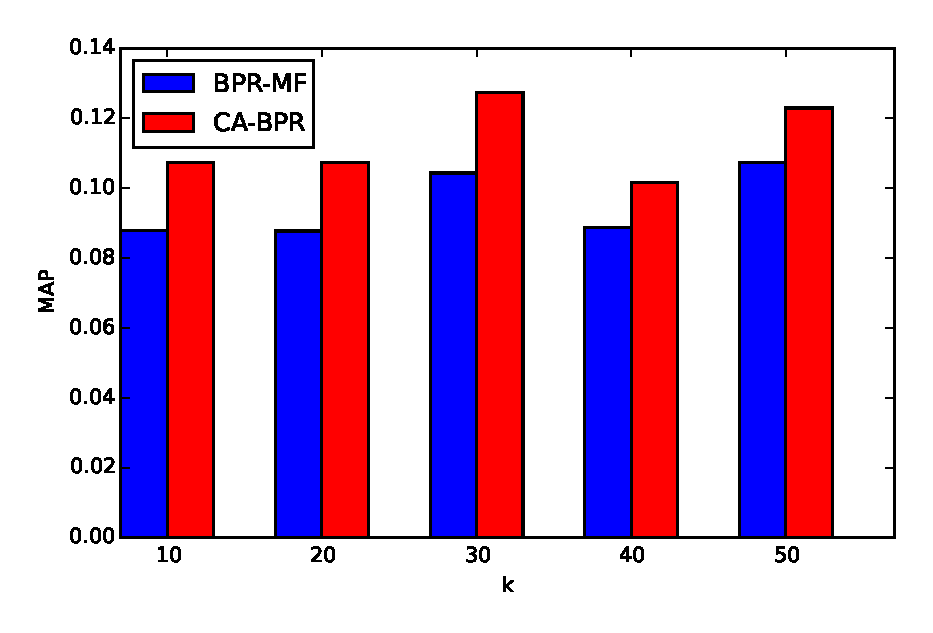
\includegraphics[width=3in]{bar}
		\end{center}
		\caption{CA-BPR indeed performs better than BPR-MF.}
	\end{figure}
\end{frame}

\begin{frame}
	\centering
	\Huge Thank you !
\end{frame}
	\section{融合内容信息的适应性BPR}
在上述章节中, 我们阐述了如何通过一个适应性采样策略加快BPR的学习, 同时通过仅考虑隐式反馈学习了the latent factors of entities。 不过, 在现实世界的推荐系统中, 很可能没有足够的协同信息, 比如, 新的物品可能会在任何时间被加入到推荐系统中。因此, 我们提出一个更为全面的个性化推荐方法:Content-aware and Adaptive Bayesian Personalized Ranking, 它基于上面所提出的适应性采样策略, 同时将隐式反馈与内容信息融合入一个统一的推荐框架中.


\subsection{Learning Content-aware Mappings}
我们首先正提出一个对于学习content-aware mappings的一个非监督解决方案。用矩阵$A^e = \left[a_1^e,a_2^e,a_3^e,\dots\right]$来表示content features of entities.然后我们提出对于学习content-aware mappings的目标函数:
\begin{equation}
L_{content} = \| A^eW^e - Y^e\|_F^2
\end{equation}
这里的$W^e \in \mathbb{R}^{d^e \times k}$表示映射矩阵(mapping matrix), $k$表示latent vectors的维度。




\subsection{Parameter Inference of CA-BPR}
通常来讲, 由于缺乏监督信息(supervised information),在公式所表述的优化问题并无确定解法。不过, 根据子空间的研究, 我们可以从隐式反馈中学习一个latent matrix $\widetilde{Y^e}$, 并用$\widetilde{Y^e}$近似代替$Y^e$. 因此, 将$\widetilde{Y^e}$代替$Y^e$代入公式, 那么目标函数变为: 
\begin{equation}
L_{content} = \| A^eW^e - \widetilde{Y^e}\|_F^2
\end{equation}

使用$\widetilde{Y^e}$近似代替$Y^e$不仅能够优化目标函数, 同时还能够一起学习包含协同信息与内容信息的 $W^{e}$. 因此, 算法总体的目标函数如下:
\begin{equation}
%分隔一个过长的公式分行显示使用split环境
\begin{split}
arg \min_{\substack{\Theta, W}} L_{feedback}+L_{content}  = 
& - \sum_{\left(m,i,j\right) \in D_s} \ln f \left( r_{mij}\right) + \lambda\|\theta\|^2\\
& + \|A^eW^e-Y^e\|^2_F + \frac 12 \sum_{e\in \{u,v\}}\lambda^e\|W^e\|^2_F 
\end{split}
\end{equation}
这里的$r_{mij} = r_{mi} -r_{mj}$。
为了学习在公式中的参数$Y^u$, $Y^v$, $W^u$, $W^v$, 在每轮迭代中, 当我们更新latent factor matrix $Y^e$, 将矩阵$W^e$认为是一个常量(constant), 并将$L_{content}$视作一个正则化项(regularizer)。那么, 对于一个任意 latent parameter $\theta$ 的梯度如下:
\begin{equation}
\begin{split}
\frac{\partial L}{\partial\theta} = 
& \sum_{\left(m,i,j\right) \in D_s}\left(f\left(r_{mij}\right) - 1\right) 
\frac{\partial \left(r_{mij}\right)}{\partial \theta}\\
& + \frac{\partial \sum_{e \in \{u,v\} } \lambda^e \left(\|A^eW^e-Y^e\|_F^2\right)}{\partial \theta}   + \lambda \theta 
\end{split}
\end{equation}
对于参数$\theta$的更新公式为: $\theta = \theta - \gamma \frac{\partial L}{\partial \theta}$, 这里的$\gamma$为学习率(learning rate)。另一方面, 对于一个latent factor matrix $Y^e$, 将$Y^e$视为伪标签(pseudo labels), 并视$L_{feedback}$为常量。因此对目标求偏导:
\begin{equation}
\frac{\partial L}{\partial W^e} = \left(A^e\right)^T\left(A^eW^e-Y^e\right) + \lambda^e W^e
\end{equation} 
令$\frac{\partial L}{\partial W^e} = 0$, 那么对于$W^e$的更新公式则演变为:
\begin{equation}
\label{equ:W}
W^e = \left(\left(A^e\right)^TA^e + \lambda^e\mathbb{E}\right)A^eY^e
\end{equation}
这里的$\mathbb{E} \in \mathbb{R}^{k\times k}$表示一个单位矩阵。

总言之, 对于CA-BPR的参数学习如算法2所示.
\IncMargin{1em}
\begin{algorithm}
	\SetAlgoNoLine %不要算法中的竖线
	
	\SetKwInOut{Input}{\textbf{输入}}\SetKwInOut{Output}{\textbf{输出}}
	
	\Input{
		\\
		The observed user-item pair set $S$\;\\
		The feature matrix of items $F$\;\\
		The content features entities $A := \{A^u,A^v\}$\;\\}
	\Output{
		\\
		$\Theta \  := \{Y^u,Y^v\}$\;\\
		$W := \{W^u,W^v\}$\;\\}
	\BlankLine
	initialize the model parameter $\Theta$ and $W$ with uniform $\left(-\sqrt{6}/{k},\sqrt{6}/{k}\right)$\;
	standarized $\Theta$\;
	Initialize the popularity of categories $\rho$ randomly\;
	\Repeat
		{\text{convergence}}
		{Draw a triple $\left(m,i,j\right)$ with 算法\ref{al2}\;
			\For {each latent vector $\theta \in \Theta$}{
				$\theta \leftarrow \theta - \eta\frac{\partial L}{\partial \theta}$
			}
			
			\For {each $W^e \in W$}{
				Update $W^e$ with the rule defined in Eq.\ref{equ:W}\;
			}	
		}
		
		
	\caption{Learning paramters for BPR\label{al3}}
	
\end{algorithm}
\DecMargin{1em}

\subsection{本章小结}
本章通过学习了一个mapping矩阵利用了内容信息,同时将本文所研究的适应性采样策略融合BPR的推荐框架中,提出了CA-BPR推荐算法。
	\section{实验论证}

\subsection{数据集}
本实验采用了MovieLens\footnote{\url{http://grouplens.org/datasets/movielens/}}100k的数据集.并随机分割了数据集的80\%作为训练数据, 其余20\%作为测试数据。

\textbf{MovieLens}包含了943个用户对于1682个电影的100,000个评分数据。每个用户至少对20个电影评过分。在实验中, 用户的职业信息(occupational description)被用作用户的内容信息(content information), 电影标题中的关键词被用作电影的内容信息。与\cite{gunawardana2009unified}中的处理过程相同, 我们并不直接使用用户的等级评分数据, 而将其转化为隐式反馈数据(对电影评过分为positive, 未评过分为negative)来使用, 以此推测是否用户是否会有对电影进行评分的行为。因此, 对于一个特定的用户而言, 我们的任务就是为其预测的一个有着潜在评分可能电影的排序列表。

如图\ref{gra6}所示, MovieLens中的用户所评分过电影数目显然呈长尾分布, 有422个近一半的用户所评分过的电影个数在区间$[20, 56]$中。
\begin{figure}[htbp]
	% caption放上面就会显示在图的上方,出现在下面就是出现在图的下方
	
	\begin{center}
		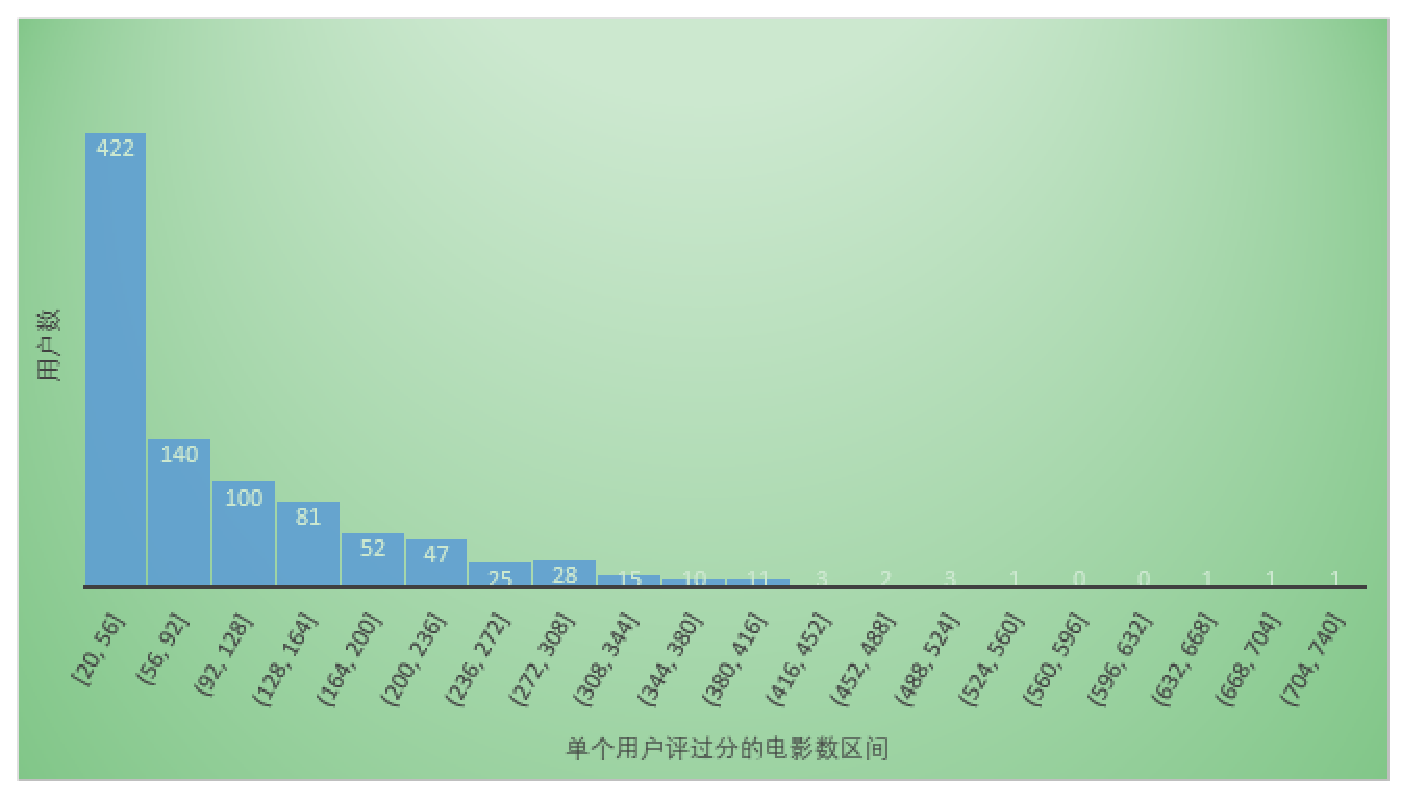
\includegraphics[width=5in]{longtail}
		\caption{用户对电影评分个数区间的长尾分布}
		\label{gra6}
	\end{center}
\end{figure}

\subsection{评测标准}

\textbf{MAP:} 先看AP(Average Precision), AP即为平均准确率。对于AP可以用这种方式理解: 假使当我们使用google搜索某个关键词,返回了10个结果。当然最好的情况是这10个结果都是我们想要的相关信息。但是假如只有部分是相关的,比如5个,那么这5个结果如果被显示的比较靠前也是一个相对不错的结果。但是如果这个5个相关信息从第6个返回结果才开始出现,那么这种情况便是比较差的。这便是AP所反映的指标,与recall的概念有些类似,不过是“顺序敏感的recall”。

对于$u$的平均准确率定义为:
\begin{equation*}
AP_u = \frac{1}{|\mathcal{I}_u^{te}|}\sum_{i \in \mathcal{I}_u^{te}}\frac{\sum_{j \in \mathcal{I}_u^{te}}\delta \left(p_{uj} \prec p_{ui}\right) + 1}{p_{ui}}
\end{equation*}
在这里$p_{ui}$表示推荐列表中物品$i$的排序位置。$p_{uj} \prec p_{ui}$表示在对用户$u$的排序列表中物品$j$的排序位置在物品$i$的前面。

对于MAP(Mean Average Precision)就很容易知道即为所有用户的AP的均值而已。那么则有:
\begin{equation*}
MAP = \frac{\sum_{u \in \mathcal{U}^{te}}AP_u}{|\mathcal{U}^{te}|}
\end{equation*}


\textbf{NDCG:}
先从CG(Cummulative Gain)说起,  CG即将每个推荐结果相关性的分值累加后作为整个推荐列表的得分。
\begin{equation*}
CG_p = \sum_{i=1}^p rel_i
\end{equation*}
在$rel_i$表示处于位置$i$的推荐结果的相关性,$p$表示所要考察的推荐列表的大小

CG的一个缺点是没有考虑结果处于不同位置对结果的影响,例如我们总是希望相关性高的结果应排在前面,相关性低的结果排在靠前的位置会严重影响用户体验, 所以在CG的基础上引入位置影响因素,即DCG(Discounted Cummulative Gain):
\begin{equation*}
DCG_p = \sum_{i=1}^p \frac{2^{rel_i}-1}{\log_2 \left(i+1\right)}
\end{equation*}

DCG仍然有其局限之处,即不同的推荐列表之间,很难进行横向的评估。而我们评估一个推荐系统,不可能仅使用一个用户的推荐列表及相应结果进行评估, 而是对整个测试集中的用户及其推荐列表结果进行评估。 那么不同用户的推荐列表的评估分数就需要进行归一化,也即NDCG(Normalized Discounted Cummulative Gain)。

IDCG(Ideal DCG)为推荐系统某一用户返回的最好结果, 即假设返回结果按照相关性排序, 最相关的结果放在最前面, 此序列的DCG为IDCG。因此DCG的值介于 $(0,IDCG]$,故NDCG的值介于$(0,1]$.

对于用户$u$的NDCG@k定义为:
\begin{equation*}
NDCG_u@k = \frac{DCG_u@k}{IDCG_u}
\end{equation*}

那么,则有:
\begin{equation*}
NDCG@k = \frac{\sum_{u\in \mathcal{U}^{te}}NDCG_u@k}{|\mathcal{U}^{te}|}
\end{equation*}

在具体操作中, 可以事先确定推荐目标和推荐结果的相关系分级, 例如可以使用 0,1分别表示相关或不相关,比如此处我们用$ref_i = \delta \left( i \in \mathcal{I}_u^{te}\right)$ , 在这里如果$x$为true, 则$\delta\left(x\right) = 1$,否则$\delta \left(x\right) = 0$. 或是这是0~5分别表示严重不相关到非常相关, 也即相当于确定了$rel$值的范围。之后对于每一个推荐目标的返回结果给定$rel$值,然后使用DCG的计算公式计计算出返回结果的DCG值。使用根据排序后的$rel$值序列计算IDCG值, 即可计算NDCG.

\subsection{实验过程与分析}
我们对BPR-MF与CA-BPR分别就MAP与NDCG评测指标进行了比较。BPR-MF\cite{rendle2009bpr}应用了矩阵分解的BPR算法框架,同时采用均匀采样策略选取训练采样。CA-BPR\cite{DBLP:conf/webi/GuoWWT15}在利用了隐式反馈数据的基础上同时融入了内容信息,并采取非均匀的适应性采样策略。

表\ref{tab:characteristic}显示了实验方法的不同之处。
\begin{table}[htbp]
	\caption{BPR-MF与CA-BPR方法特征比较}
	\renewcommand\arraystretch{1.3}%改变行高
	\label{tab:characteristic}
	\begin{center}
		\begin{tabular}{|c|c|c|}
			\hline
			Method   &   Content & Sampling   \\
			\hline
			BPR-MF   &   no      & uniform    \\
			CA-BPR   &   yes     & non-uniform\\
			\hline
			
		\end{tabular}
	\end{center}
\end{table}

表\ref{tab:mapandndcg}显示了BPR-MF与CA-BPR的MAP与NDCG实验结果。
\begin{table}[htbp]
	\caption{不同维度k下算法MAP与NDCG实验结果}
	\label{tab:mapandndcg}
	\begin{center}
		\begin{tabular}{|c | c |c |c|c|c|}
			\hline
			BPR-MF  &   k=10 &   k=20 &    k=30&    k=40&    k=50\\
			\hline
			MAP      &  0.0879&  0.0877&  0.1043&  0.0888&  0.1074\\
			\hline
			NDCG@3   &  0.3051&  0.3545&  0.3398&  0.2491&  0.3790\\
			NDCG@5   &  0.3616&  0.4296&  0.3708&  0.2984&  0.4153\\
			NDCG@10  &  0.4120&  0.4632&  0.4010&  0.3163&  0.4458\\
			NDCG@20  &  0.4121&  0.4575&  0.4164&  0.3415&  0.4323\\
			\hline
		\end{tabular}
		
	\end{center}
\end{table}
\begin{table}[htbp]
		\vspace{-1em}
		\begin{center}
			
		\begin{tabular}{|c | c |c |c|c|c|}
			\hline
			CA-BPR  &     k=10&   k=20 &    k=30&  k=40 &   k=50  \\
			\hline
			MAP     &   0.1074&  0.1072&  0.1274&  0.1016&  0.1229\\
			\hline
			NDCG@3  &   0.3790&  0.4336&  0.4152&  0.3044&  0.4631\\
			NDCG@5  &   0.4153&  0.4752&  0.4531&  0.3646&  0.5074\\
			NDCG@10 &   0.4458&  0.5101&  0.4900&  0.3865&  0.5447\\
			NDCG@20 &   0.4323&  0.4946&  0.5088&  0.4173&  0.5282\\
			\hline
		\end{tabular}
	\end{center}
\end{table}

图\ref{fig:map}显示了BPR-MF与CA-BPR在不同维度下的MAP结果对比。显然,融合了内容信息同时采用适应性采样策略的CA-BPR推荐效果比BPR-MF要好,由此说明内容信息及适应性采样策略的确是有效的。
\begin{figure}[htbp]
	\begin{center}
	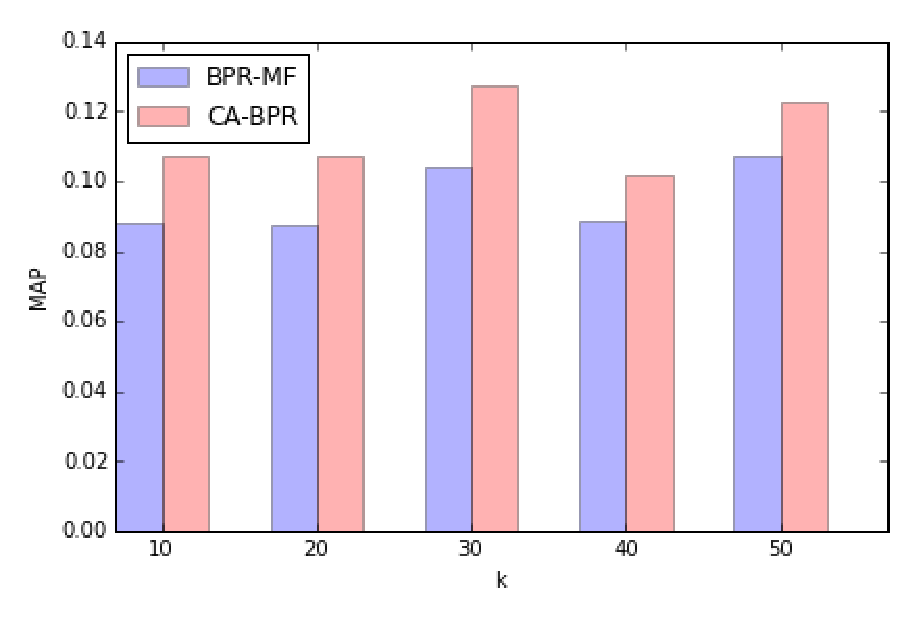
\includegraphics[width=4in]{mapbar}
\end{center}
\caption{不同维度算法MAP结果对比}
\label{fig:map}
\end{figure}

	\section{结论与展望}

\subsection{本文的主要内容}

本文首先回顾了采用均匀采样策略的经典BPR推荐算法,然后分析其在随机梯度学习算法中导致收敛缓慢的原因。而后在隐式反馈的基础上加入内容信息提出了非均匀的适应性采样策略,并将其融入BPR推荐框架中。实验证明本文所研究的方法的确能够提高推荐效果。

\subsection{进一步的研究工作}
尽管本文实验证明通过加入内容信息的确有助于提高推荐效果,但是对于加入内容信息的适应性采样策略在整个学习过程每个阶段的影响仍然有待研究。同时对于一些已有的一些融合内容信息的推荐方法,比如采用Word2Vec技术,还需进一步的研究调查在这些融合内容信息的不同推荐方法中的特点,适用性及其局限性。
	
	
	%参考文献
	\kaishu
	\bibliographystyle{plain}
	\addcontentsline{toc}{section}{参考文献} %向目录中添加条目,以章/section的名义
	\bibliography{ref/szuthesis.bib}
	
	
	%致谢与英文摘要
	\fangsong
	\newpage

\section*{\centerline{\heiti\zihao{-4}{致谢}}}
\addcontentsline{toc}{section}{致谢}

首先衷心地感谢潘微科老师。在本科生涯最后的一年多里,不仅是现时的学业与学术, 更是对于未来的发展给予了我很多指导与帮助。本次毕业设计,从选题到论文撰写,给予了我很多宝贵的意见。他渊博的学识、严谨的治学态度及认真负责的工作态度都使我受到鼓舞和熏陶。在此向潘微科老师表示崇高的敬意和衷心的感谢, 他的言传身教将使我终生受益。

\vspace{5bp}
感谢key哥哥与在453认识的朋友们, 与你们的交流大概就是我对计算机启蒙的开始. 如果不是有幸与你们相识, 这一路走来必是要曲折地多.

\vspace{5bp}
感谢 Thuthesis 及其作者薛瑞尼. 最终虽未使用Thuthesis模板, 但是此间对其研习所得对我顺利使用 \LaTeX 完成论文撰写仍然起了很大作用.

\vspace{5bp}
感谢一直关心我的父母与兄长。远游在外, 感谢还有你们牵挂.

\vspace{5bp}
感谢自己熬过了那段难捱的日子。从学习画画到广播电视再到计算机科学, 在如今看来似曾是做了诸多无用功, 不过幸而没有因为短时的平庸迷茫而消磨掉满心的戾气. 

\vspace{5bp}
前路漫漫, 不冀求大步流星, 唯盼能步步坚实.
	\newpage

\centerline{\fangsong\bf\zihao{-2}{Research on Content-Aware Collaborative Filtering }}

\addcontentsline{toc}{section}{Abstract(Key words)}

\vskip 20bp

\hspace{4bp} {\zihao{-4}\textbf{【 Abstract】}} 
Pairwise learning algorithms are a vital technique
for personalized ranking with implicit feedback. They usually
assume that each user is more interested in items which have
been selected by the user than remaining ones. This pairwise
assumption usually derives massive training pairs. To deal with
such large-scale training data, the learning algorithms are usually
based on stochastic gradient descent with uniformly drawn pairs.
However, the uniformly sampling strategy often results in slow
convergence. In this paper, we first uncover the reasons of
slow convergence. Then, we associate contents of entities with
characteristics of dataset to develop an adaptive item sampler
for drawing informative training data. In this end, to devise a
robust personalized ranking method, we accordingly embed our
sampler into Bayesian Personalized Ranking (BPR) framework,
and further propose a Content-aware and Adaptive Bayesian
Personalized Ranking (CA-BPR) method, which can model both
contents and implicit feedbacks in a unified learning process. The
experimental results show that our adaptive item sampler can indeed improve recommendation performance.

\vskip 10bp

\hspace{5bp}{\zihao{-4}\textbf{【 Keywords】}}
Recommendation System; Collaborative Filtering; Adaptive Sampling


\vskip 20bp

\begin{flushright}
	\kaishu指导教师:\ 潘微科 \hspace{3cm}{ }
\end{flushright}

\label{lastpage}%%%%显示总页数
\end{document}